\documentclass[ngerman, 12pt, pdftex]{scrartcl}[2006/07/30]

%encoding and input
\usepackage[ngerman]{babel} %spell correction
\usepackage[latin1]{inputenc} 
\usepackage[T1]{fontenc}

%bugfixes
\usepackage{fixltx2e} 

%Font Symbols and Colors
\usepackage{textcomp} %more symbols
\usepackage{xcolor}

%Math
\usepackage{amsmath}
\usepackage{mathtools} %extends amsmath

%Programming
\usepackage{listingsutf8} %in utf8
\lstset{language=Java,captionpos=b,tabsize=3,frame=lines,keywordstyle=\color{blue},commentstyle=\color{teal},stringstyle=\color{red},numbers=left,numberstyle=\tiny,numbersep=5pt,breaklines=true,showstringspaces=false,basicstyle=\footnotesize,emph={label},upquote=true} %Syntax highlighting

%Verbatim extension (with line numbers and tab-expansion)
\usepackage{moreverb} 

%Headers and Footer
\usepackage{fancyhdr}

%title
\title{Handbuch}
\author{Frank M\"{u}ller, Oliver Wisler, Luzius Bachmann, Fabio Sulser}
\subtitle{Swissdefcon-Team}

\begin{document}
%declare  Header
\pagestyle{fancy}
\fancyhf{} 
\fancyhead[L]{Handbuch} %left header
\fancyhead[C]{Swissdefcon-Team} %centered header
\fancyhead[R]{\thepage}  % right header
\renewcommand{\headrulewidth}{0.1pt} 	%upper separating line
\fancyfoot[C]{\thepage} 				%centered footer, line number



%you might want to enable come features:
\maketitle
%\listoffigures 
%\listoftables


\newpage

\tableofcontents

\newpage

\section{Anmeldung}

Starte das Spiel und melde dich volgendermassen an.

\begin{figure}[h]
\centering
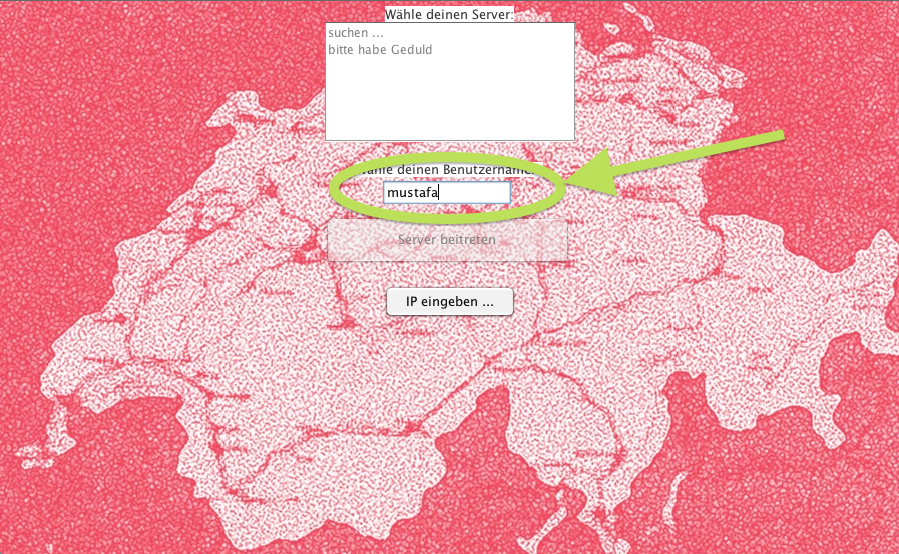
\includegraphics[scale=0.3]{starten/namen_eingeben.png}
\caption{Gib den Namen ein}
\end{figure}

Gib in dem Markierten Feld den Namen ein. Standardm\"{a}ssig wird der Name deines Computers verwendet.

\begin{figure}[h]
\centering
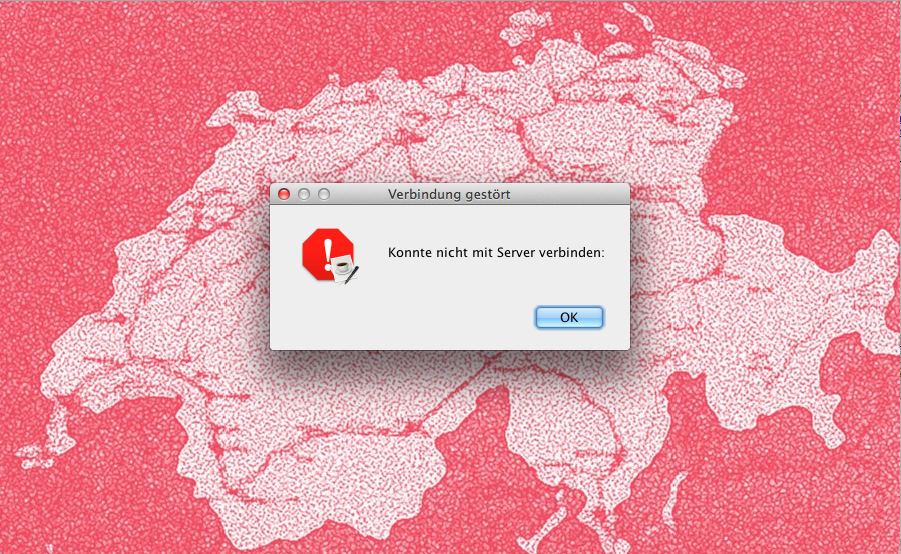
\includegraphics[scale=0.3]{starten/keine_serververbindung.png}
\caption{Error, keine Verbinfung zum Server}
\end{figure}

Falls du keine Verbindung zum Server hast wird die Obige Meldung angezeigt.

\newpage

\begin{figure}[h]
\centering
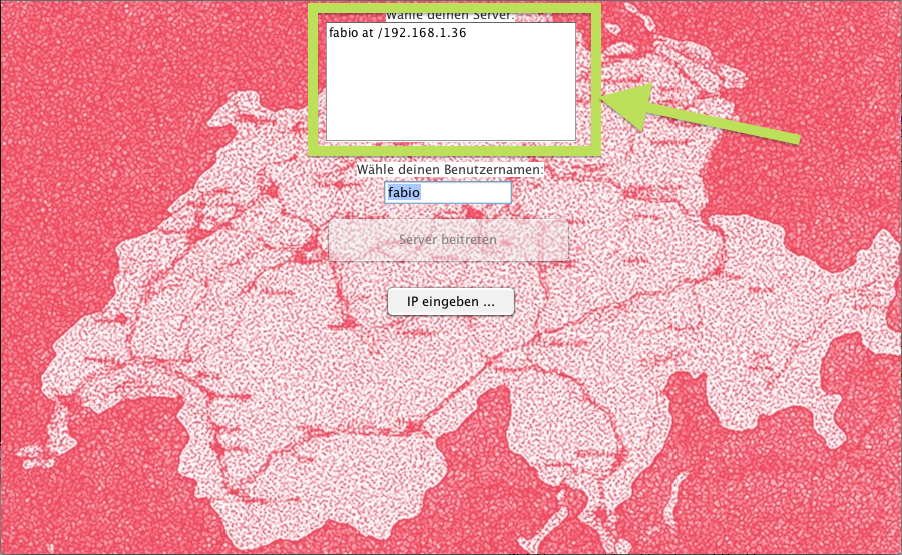
\includegraphics[scale=0.3]{starten/serverliste.png}
\caption{Liste der Server}
\end{figure}

In dem oben marierten Feld siehst du die Liste der aktiven Server.

\begin{figure}[h]
\centering
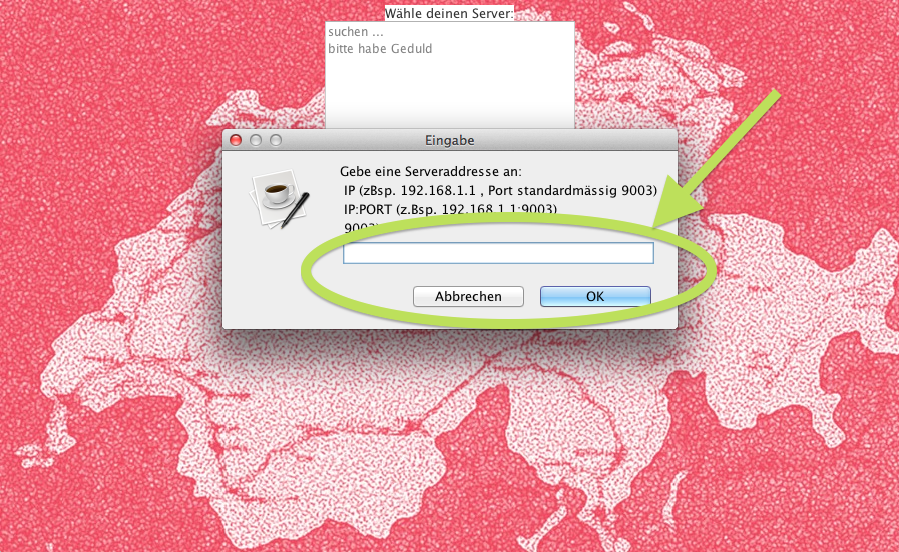
\includegraphics[scale=0.3]{starten/IP_manuell_eingeben.png}
\caption{Serveradresse eingeben}
\end{figure}

Gibt es einen Server, der nicht in der Liste angezeigt wird, so kannst du dessen Adresse auch per
Hand eingeben.

\newpage

\begin{figure}[h]
\centering
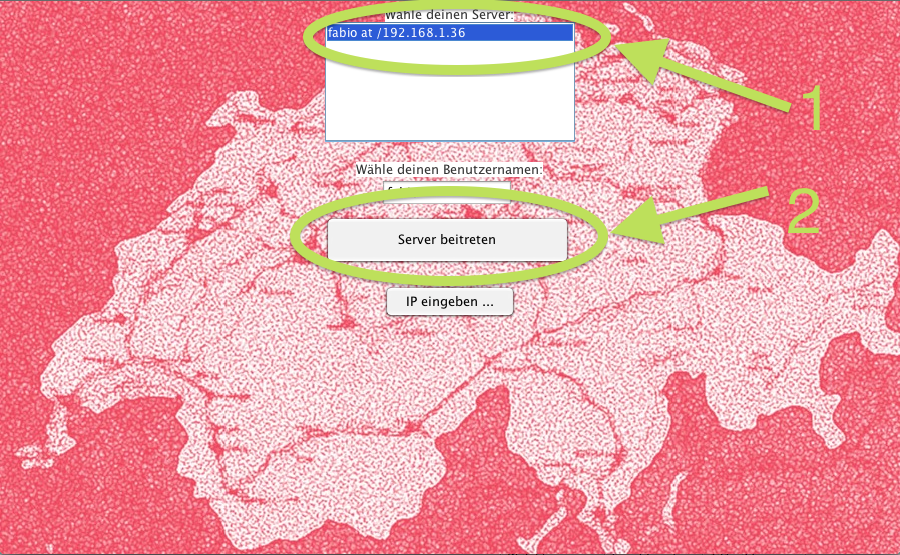
\includegraphics[scale=0.3]{starten/server_waehlen.png}
\caption{Server w\"{a}hlen}
\end{figure}

W\"{a}hle einen Server aus der ober beschriebenen Liste per Mausklick aus un gib deinen(1) und dr\"{u}cke dann auf "'Server betreten"'(2).



\end{document}
